\chapter{Families of plane algebraic curves}

\epigraph[author={Leo Tolstoy}, source={Anna Karenina}]{All happy families are alike; each unhappy family is unhappy in its own way.}\SubIndex{Tolstoy, Leo}\SubIndex{Karenina, Anna}

\section{Pencils of curves}
Take two curves \(B\) and \(C\) of the same degree \(n\), with equations \(b(x,y)=0\) and \(c(x,y)=0\).
The level sets 
\[
\frac{b(x,y)}{c(x,y)} = r
\]
of the ratio form a collection of curves \(C_r\), called the \emph{pencil}\define{pencil} of curves containing \(B\) and \(C\).
The curve \(B\) is \(C_0\) while \(C\) is \(C_{\infty}\).
Every point in the projective plane lies on a unique one of these curves, with value \(r\) given by taking the value of the homogenized \(b(x,y,z)/c(x,y,z)\) at that point, except for the points in \(B \cap C\), for which the ratio is never defined.
To be more precise, each curve \(C_r\) can also be written as
\[
b(x,y) = r \, c(x,y),
\]
(except for \(C_{\infty}=C\)).
The points of \(B \cap C\) belong to \emph{all} curves \(C_r\) of the pencil.
Moreover the degree of \(C_r\) is the same as that of \(B\) and \(C\).
\begin{example}
The lines through a point form a pencil: if \(B=(x=0)\) and \(C=(y=0)\) then \(C_r =(x=ry)\).
\begin{center}
\documentclass[11pt]{standalone}
\usepackage{xparse}
\usepackage{tikz}
\colorlet{curveZero}{gray!85}
\colorlet{curveOne}{blue!60}
\definecolor{curveOneColor}{rgb}{.6,0,0}
\colorlet{curveTwo}{brown!50!gray}
\colorlet{curveThree}{green!40!gray}
\colorlet{curveFour}{red!50!gray}
\NewDocumentCommand\DrawDotInPlot{O{}mmO{}}%
{%
\fill[gray!15,draw=gray] (axis cs:{#2},{#3}) circle [radius=1.6pt] node[above,black,#4] {\(#1\)};%
}%
\NewDocumentCommand\DrawDot{O{}mmO{}}%
{%
\fill[gray!20,draw=gray] ({#2},{#3}) circle (1.6pt) node[above,black,#4] {\(#1\)};%
}%
\NewDocumentCommand\DrawNode{O{}m}%
{%
\fill[gray!20,draw=gray] (#2) circle (1.6pt) node[above,black] {\(#1\)};%
}%
\NewDocumentCommand\DrawDotThreeD{O{}mmmO{}}%
{%
\fill[gray!20,draw=gray] ({#2},{#3},{#4}) circle (1.6pt) node[above,black,#5] {\(#1\)};%
}%
\colorlet{axisColor}{gray!50}
\tikzstyle{shapeZero}=[fill=curveZero,opacity=.4]
\tikzstyle{shapeOne}=[fill=curveOne,opacity=.4]
\tikzstyle{shapeTwo}=[fill=curveTwo,opacity=.4]
\tikzstyle{shapeThree}=[fill=curveThree,opacity=.4]
\tikzstyle{groupElementLabel}=[minimum size=2.4em]
\tikzstyle{groupElement}=[minimum size=2.4em,shapeZero,draw=curveZero]
\tikzstyle{cosetOne}=[minimum size=2.4em,shapeOne,draw=curveOne]
\tikzstyle{cosetTwo}=[minimum size=2.4em,shapeTwo,draw=curveTwo]


\begin{document}
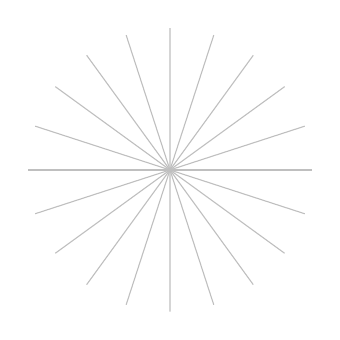
\begin{tikzpicture}
\newcommand{\RRR}{1.8}
\foreach \i in {0,...,9}
{
\draw[axisColor] 
		({\RRR*cos(3.1415*\i/10 r)},{\RRR*sin(3.1415*\i/10 r)}) 
	-- ({-\RRR*cos(3.1415*\i/10 r)},{-\RRR*sin(3.1415*\i/10 r)});
}
\DrawDot{0}{0}
\end{tikzpicture}
\end{document}

\end{center}
\end{example}
\begin{example}
The pencil of conics containing the circle \(x^2+y^2=1\) and the reducible conic \(x^2=y^2\) (which is a pair of lines \(x=\pm y\)):
\[
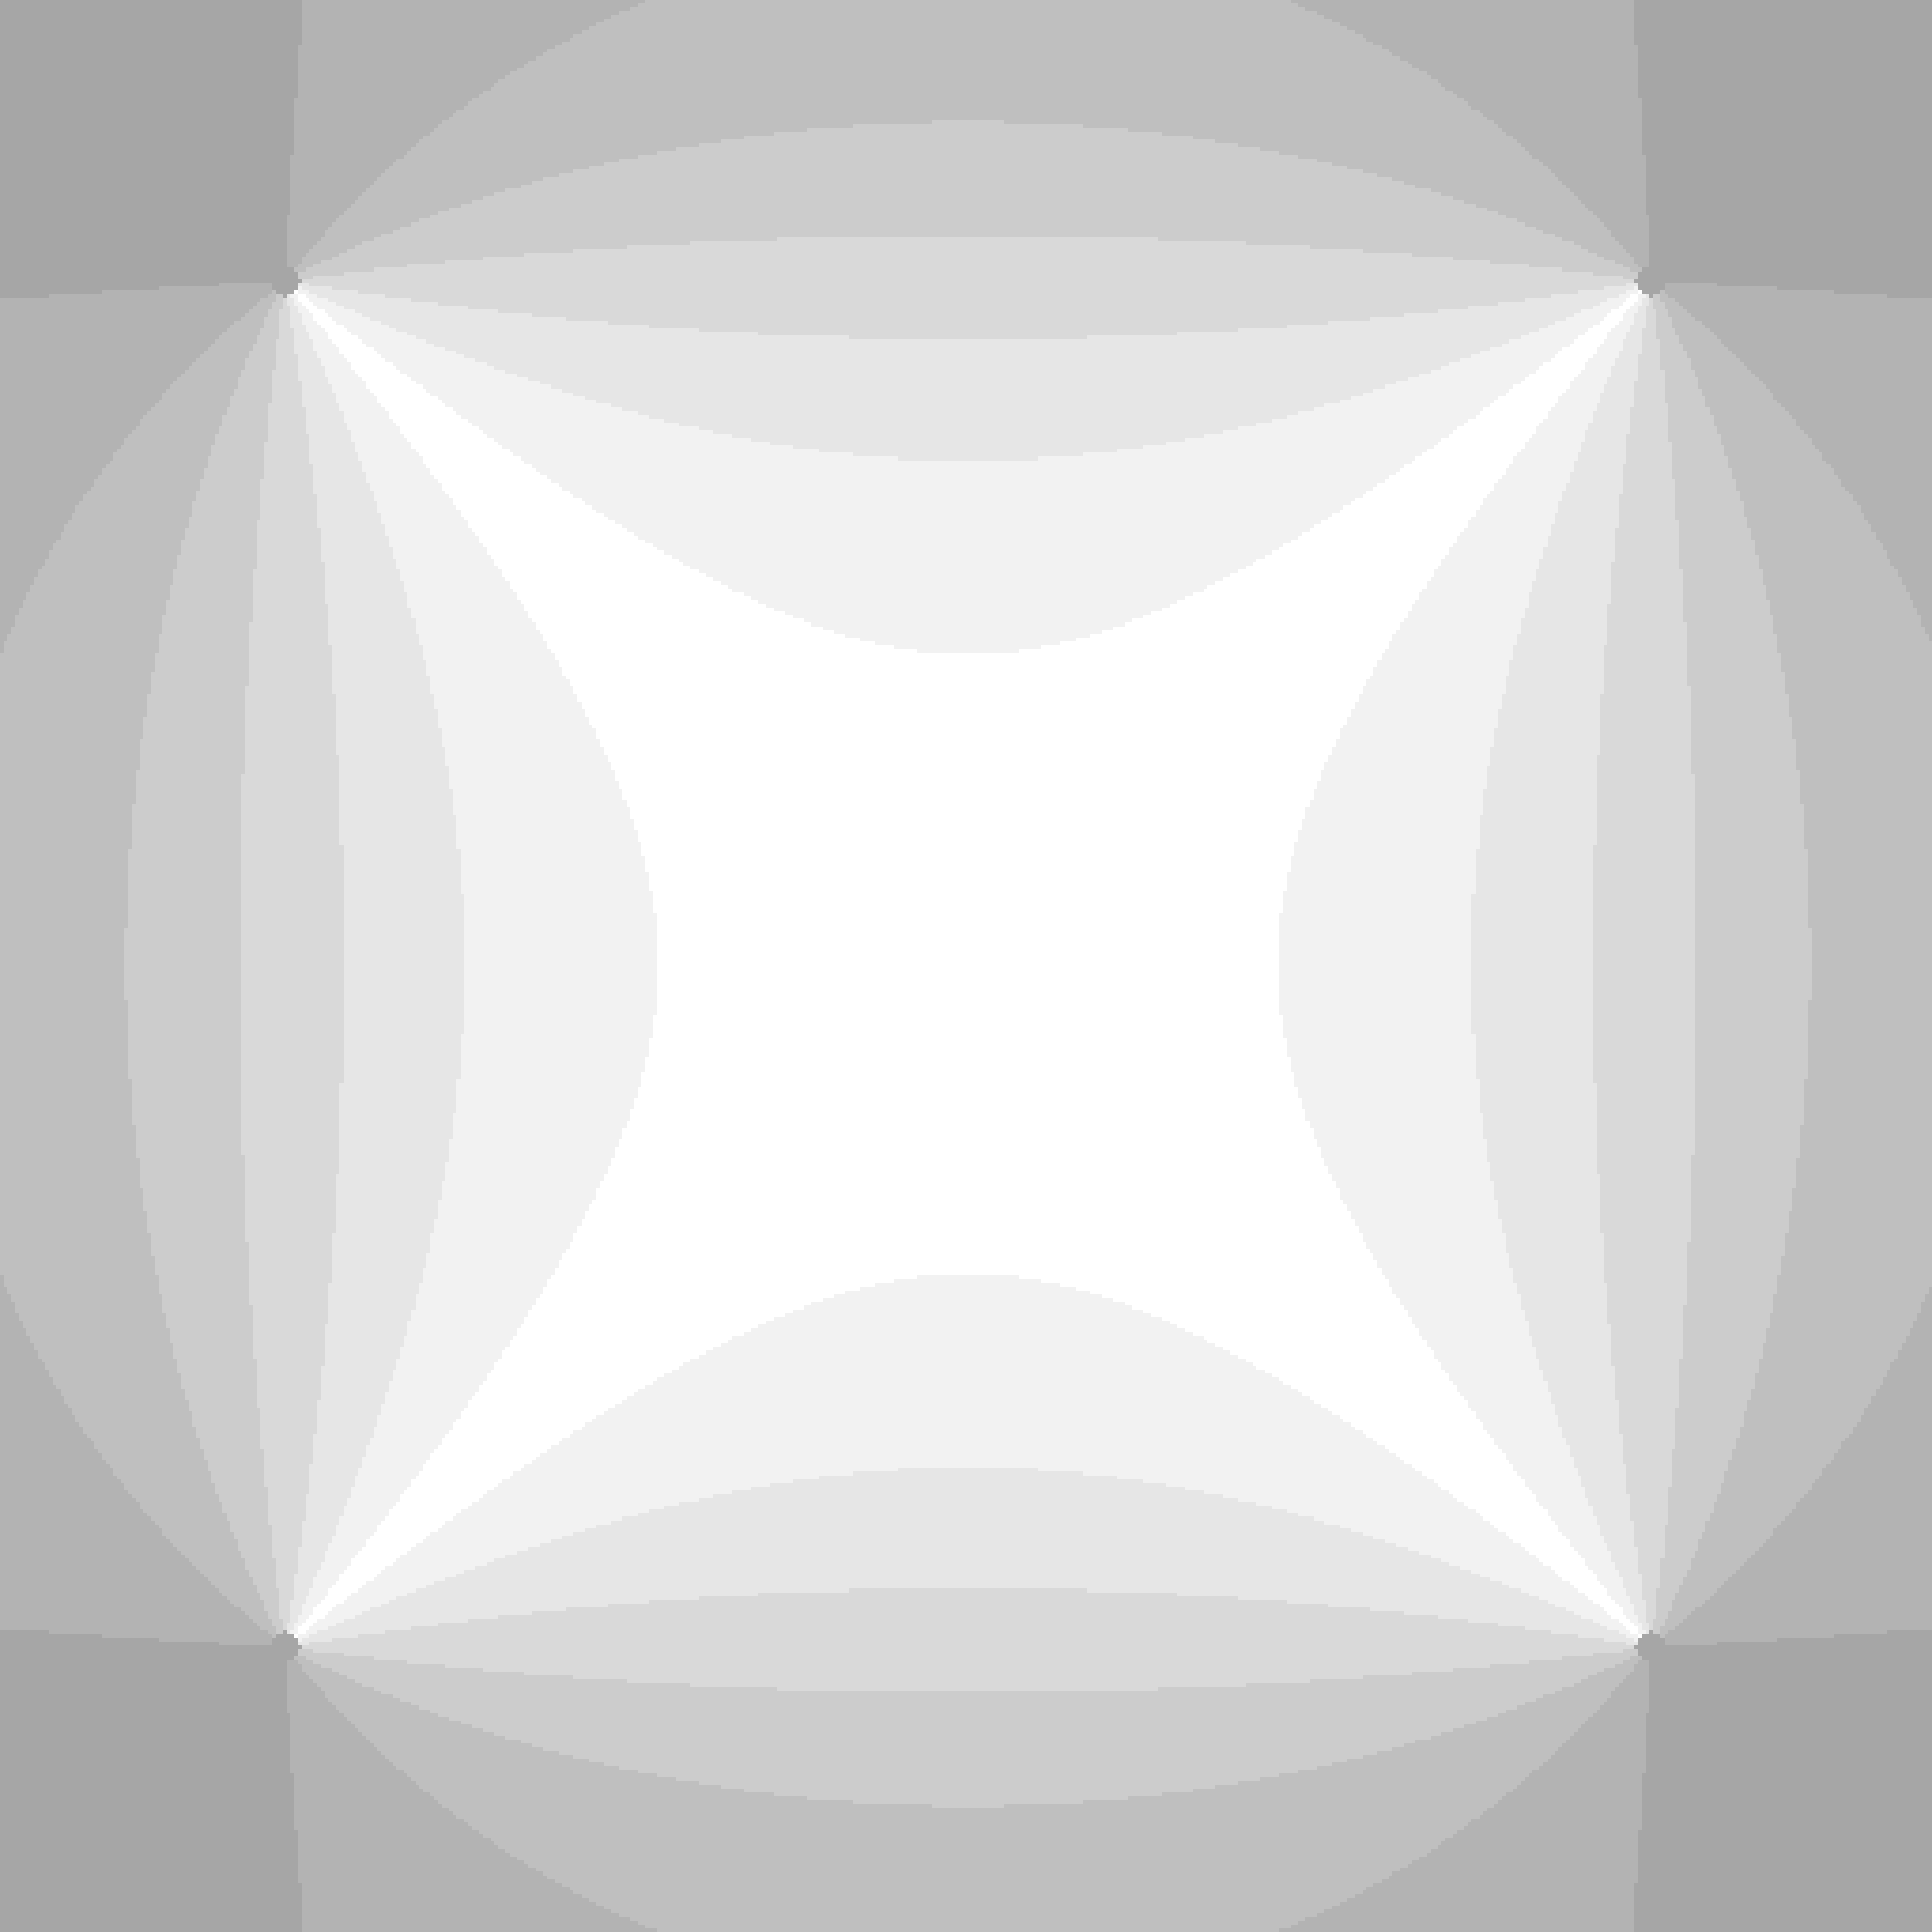
\includegraphics[width=4cm]{pencils/pencil-1}
\]
Look at the 4 points where the circle intersects the two lines; these points lie in every conic in the pencil.
\end{example}
\begin{example}
The pencil of cubics containing \(y^2=x+x^3\) and \(xy^2=0\):
\[
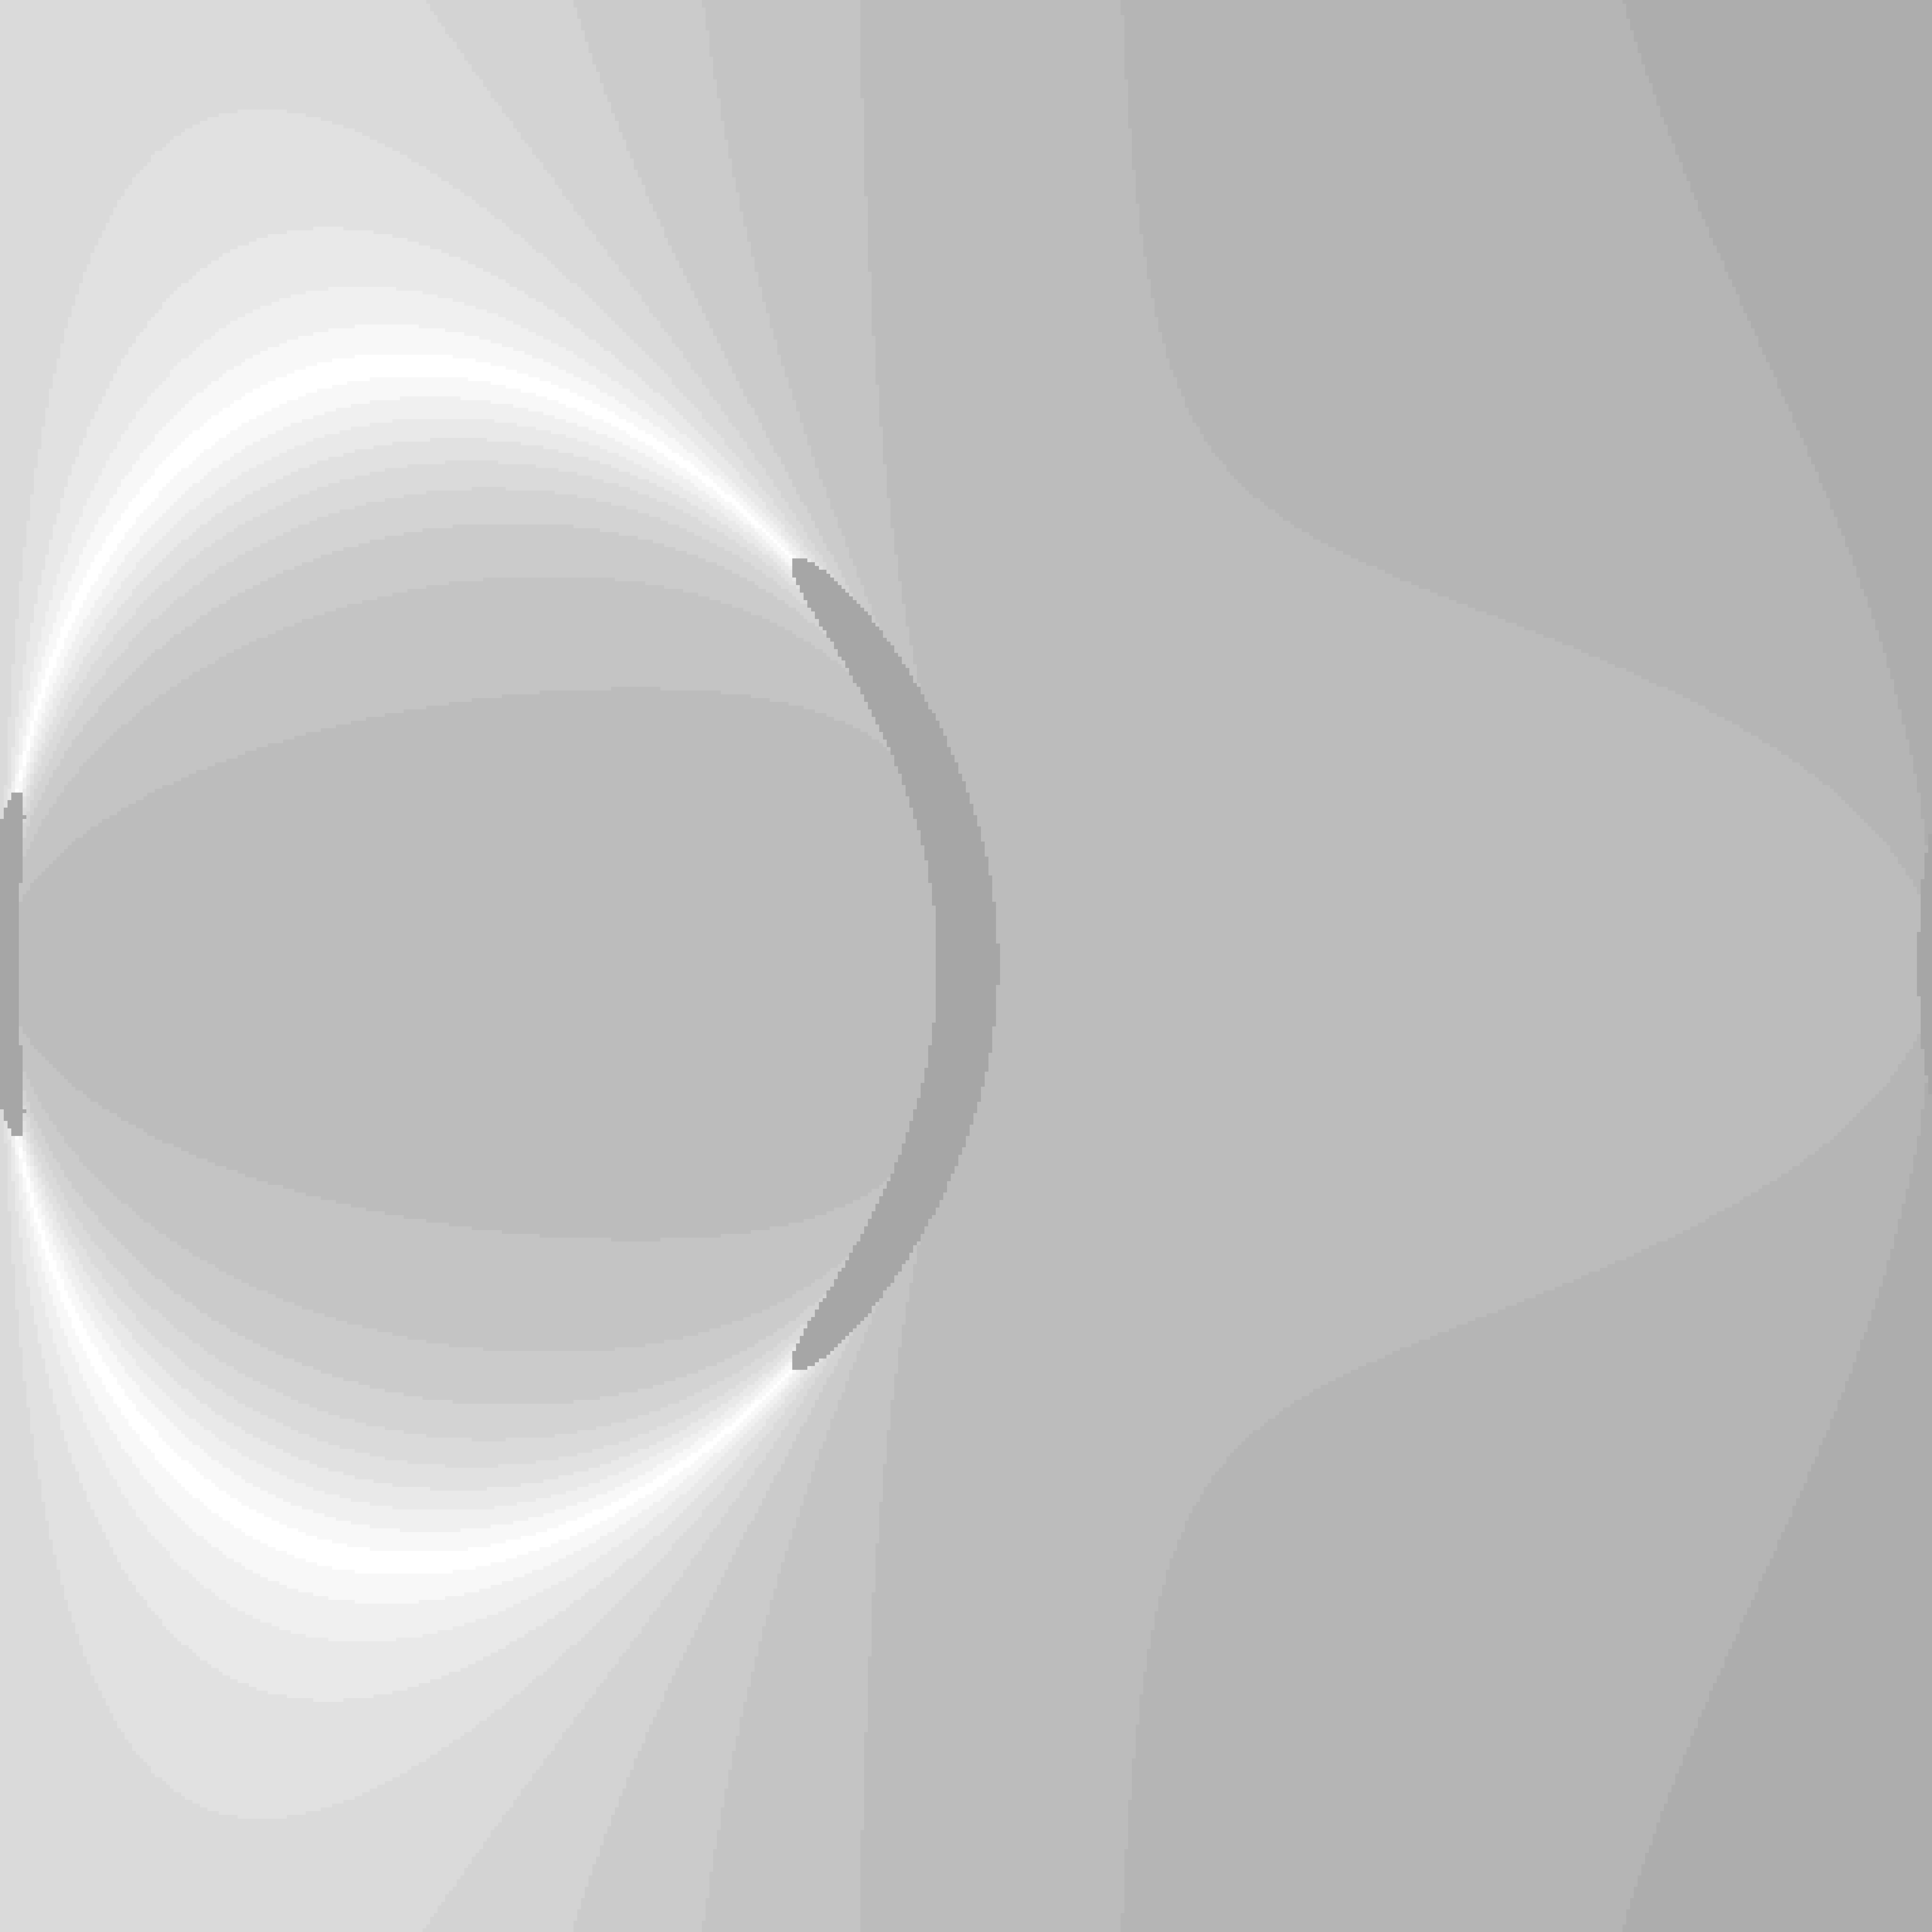
\includegraphics[width=4cm]{pencils/pencil-2}
\]
\end{example}
\begin{example}
\emph{Danger}: for some values of \(r\), \(C_r\) might actually be of lower order than \(B\) or \(C\).
For example, if \(B=(y^2=x)\) and \(C=(-y^2=x)\), two conics, the pencil has curves \(C_r\) with equation
\[
\pr{1-r}y^2=(1+r)x,
\]
which drops order at \(r=1\), i.e. \(C_1\) is a line.
But note that if we homogenize,
\[
\pr{1-r}y^2=(1+r)zx,
\]
the curve \(C_1\) is actually a pair of lines.
In a pencil \(C_r\) for which \(C_0\) and \(C_{\infty}\) are irreducible, we rarely but occasional find reducible curves, as in this example, and we might picture that the moving curve \(C_r\) ``bubbles'' into reducible components.
\begin{center}

\includegraphics[width=3cm]{Girl_blowing_bubbles.jpg}
\par\noindent{\tiny{Creative Commons license, Attribution NonCommercial Unported 3.0, Fir0002/Flagstaffotos}}
\end{center}
\end{example}
\section{Zeroes and poles}
If \(f(x,y,z)\) is a rational function, say
\[
f(x,y,z)=\frac{b(x,y,z)}{c(x,y,z)},
\]
then the level sets of \(f(x,y,z)\) are the curves 
\[
C_r=(f(x,y,z)=r)=(b(x,y,z)=rc(x,y,z))
\]
of the linear system with \(C_0=(f=0)\) and \(C_1=(1/f=0)\).
Suppose that \(D\) is a plane algebraic curve so that \(f\) is not constant on any component of \(D\).
Then the level set \(C_r\) intersects it with intersection number 
\[
\degree{D}\degree{C_r}=\degree{D}\degree{f}
\]
where \(\degree{f}\) means \(\degree{p}\), which also equals \(\degree{q}\).
In particular, counting with multiplicity, all level sets of \(f\) strike the curve \(D\) at the same number of points.
Define the \emph{order} of \(f\) at a point \(p\) of \(D\) to be \(\multiplicity{p}{C_0}{D}\) and the \emph{order of pole} of \(f\) to be \(\multiplicity{p}{C_0}{D}\).
In particular, there are as many zeroes of \(f\) on \(D\) as poles, counted with their orders.

\section{Making bubbles}
\begin{lemma}\label{lemma:bubble}
Suppose that two projective plane algebraic curves \(B\) and \(C\) of the same degree \(n\) intersect at exactly \(n^2\) points (the maximum possible by B\'ezout's theorem).
Write \(n\) as \(n=p+q\).
If exactly \(pn\) of these points lie on an irreducible curve \(E\) of degree \(p\) (again the maximum possible) then the remaining points, \(qn\) of them, lie on a curve \(F\) of degree \(q\) (again the maximum possible).
\end{lemma}
\begin{proof}
Write \(B\) and \(C\) as \(C_0\) and \(C_{\infty}\) in a pencil \(C_r\).
Pick a point \(s\) of \(E\) different from the intersection points of \(C_0\) and \(C_{\infty}\); by problem~\vref{problem:intersecting.curves:nonzero.somewhere.4}, there are infinitely many.
The point \(s\) then belongs to a unique element of the pencil, say to \(C_{r_0}\).
Then \(s\) sits in \(C_{r_0}\) along with all of the points of \(B \cap C\) and \(s\) also sits in \(E\) along with \(pn\) points of \(B \cap C\).
So \(E\) and \(C_{r_0}\) contain the same \(1+pn\) points of \(B \cap C\).
By B\'ezout's theorem, as the degrees of \(E\) and \(C_{r_0}\) are \(p\) and \(n\), they contain a common irreducible component.
Since \(E\) is irreducible by assumption, \(E\) is that component of \(C_{r_0}\).
So \(C_{r_0} = E \cup F\), for some curve \(F\) of degree at most \(q\), i.e. the pencil bubbles into two components.
The remaining intersection points of \(B \cap C\) don't lie in \(E\), but all lie in \(C_{r_0}\), so they lie in \(F\).
\end{proof}

\section{Polygons}\label{section:polygons}
A \emph{quadrilateral}\define{quadrilateral} is a quadruple of points, called the \emph{vertices}, no three on the same line, with a chosen ordering defined up to cyclically permuting, so there is no first point or second point, but if you pick a point from the quadruple, there is a next point, and a next, and so on until you come back to the point you started with.
In the same way, we define a \emph{polygon}\define{polygon}.
The lines through subsequent vertices are the \emph{edges}.
We can't define the notion of a square or rectangle since there is no notion of length or angle available.

\section{Pascal's mystic hexagon}
\begingroup
\newcommand*{\drawEllipse}
{
\draw[very thick,curveZero] (0,0) ellipse (1cm and .5cm);
}
\newcommand*{\drawHexagon}
{
\foreach \i in {0,...,5}
	{
	\newcommand*{\dd}{8}
		\coordinate (p\i) at ({cos(20*\i+\dd*\i*\i)},{.5*sin(20*\i+\dd*\i*\i)}) {};
		\DrawNode{p\i}
	}
}
\newcommand*{\findFirstIntersection}
{
\coordinate (c1) at (intersection of p0--p1 and p3--p4) {};
}
\newcommand*{\findSecondIntersection}
{
\coordinate (c2) at (intersection of p1--p2 and p4--p5) {};
}
\newcommand*{\findThirdIntersection}
{
\coordinate (c3) at (intersection of p2--p3 and p5--p0) {};
}
\newcommand*{\findAllIntersections}
{
\findFirstIntersection
\findSecondIntersection
\findThirdIntersection
}
% highest x value of any coordinate of any point in the picture:
\newcommand*{\maxX}{3.5}
% lowest x value of any coordinate of any point in the picture:
\newcommand*{\minX}{-1}
\newcommand*{\showTheLine}
{
\begin{scope}[on background layer]
\draw[curveThree,very thick] (c1) -- (c3);
\draw[curveThree,very thick] (c3) -- (c2);
\end{scope}
}
\newcommand*{\firstPicture}
{
\drawEllipse
\drawHexagon
\begin{scope}[on background layer]
\draw[curveOne,very thick] (p1) -- (p2);
\draw[curveOne,very thick] (p2) -- (p3);
\draw[curveOne,very thick] (p3) -- (p4);
\draw[curveOne,very thick] (p4) -- (p5);
\draw[curveOne,very thick] (p5) -- (p0);
\draw[curveOne,very thick] (p0) -- (p1);
\end{scope}
}
\newcommand*{\secondPicture}
{
\firstPicture
\findFirstIntersection
\begin{scope}[on background layer]
\draw[curveTwo,very thick,opacity=.5] (p1) -- (c1);
\draw[curveTwo,very thick,opacity=.5] (p3) -- (c1);
\end{scope}
\DrawNode{c1}
}
\newcommand*{\thirdPicture}
{
\firstPicture
\findSecondIntersection
\begin{scope}[on background layer]
\draw[curveTwo,very thick,opacity=.5] (p1) -- (c2);
\draw[curveTwo,very thick,opacity=.5] (p5) -- (c2);
\end{scope}
\DrawNode{c2}
}
\newcommand*{\fourthPicture}
{
\firstPicture
\findThirdIntersection
\begin{scope}[on background layer]
\draw[curveTwo,very thick,opacity=.5] (p2) -- (c3);
\draw[curveTwo,very thick,opacity=.5] (p0) -- (c3);
\end{scope}
\DrawNode{c3}
}
\newcommand*{\fifthPicture}
{
\firstPicture
\findAllIntersections
\begin{scope}[on background layer]
\draw[curveTwo,very thick,opacity=.5] (p1) -- (c1);
\draw[curveTwo,very thick,opacity=.5] (p3) -- (c1);
\draw[curveTwo,very thick,opacity=.5] (p1) -- (c2);
\draw[curveTwo,very thick,opacity=.5] (p5) -- (c2);
\draw[curveTwo,very thick,opacity=.5] (p2) -- (c3);
\draw[curveTwo,very thick,opacity=.5] (p0) -- (c3);
\end{scope}
\DrawNode{c1}
\DrawNode{c2}
\DrawNode{c3}
}
\newcommand*{\sixthPicture}
{
\fifthPicture
\showTheLine
}
\newcommand{\Pascal}[1]{%
\par\noindent%
\begin{center}
\begin{tikzpicture}
% Draw a strut to make all of the diagrams have the same width, so the same x coordinate in each diagram gives a point the same distant across the page.
%\begin{scope}[on background layer]
\draw[white,opacity=0] (\minX,0) -- (\maxX,0); 
%\fill[gray!20,draw=black] (\minX,-3) rectangle (\maxX,4.5);
%\end{scope}
\IfStrEqCase{#1}{%
{1}%
{%%
\firstPicture
}%%
{2}%
{%
\secondPicture
}%
{3}%
{%%
\thirdPicture
}%%
{4}%
{%%
\fourthPicture
}%%
{5}%
{%%
\fifthPicture
}%%
{6}%
{%%
\sixthPicture
}%%
{7}%
{%%
\seventhPicture
}%%
{8}%
{%%
\eighthPicture
}%%
}%% end IfStrEqCase
\end{tikzpicture}
\end{center}
}

Draw a hexagon with vertices sitting inside a conic. \Pascal{1}
Since there is an even number of sides, each side has an ``opposite'' side, half way around the hexagon.
Pick a side and its opposite, and draw lines joining them. \Pascal{2}
The same for the next pair of opposite sides. \Pascal{3}
And finally for the third pair of opposite sides. \Pascal{4}
Draw all of these lines together in one picture. \Pascal{5}
Mysteriously, all three intersection points lie on a line. \Pascal{6}
\endgroup

\begin{theorem}
Given a hexagon in the projective plane over a field, the intersection points of opposite sides lie on a line.
\end{theorem}
\begin{proof}
Let \(B\) be the reducible cubic curve consisting of three of the lines, no two of them in succession (for example, the first, third and fifth lines).
Let \(C\) be the reducible cubic curve consisting of the remaining three lines of the hexagon.
Let \(E\) be the quadric.
The result follows immediately from lemma~\vref{lemma:bubble}.
\end{proof}


\section{The space of curves of given degree}
Consider the vector space \(V_d\) of homogeneous polynomials of degree \(d\) in \(3\) variables.
Each such polynomial has a coefficient of \(x^a y^b z^c\) as long as \(a+b+c=d\).
Imagine that we take \(d+2\) sticks sitting in a row.
Colour two of them white and the rest black.
Take \(a\) to be the number of black sticks before the first white one, \(b\) the number of black sticks between the two white ones, and \(c\) the number of black sticks after the second white one.
Clearly \(a+b+c=d\).
So the dimension of \(V_d\) as a vector space is 
\[
\binom{d+2}{2}.
\]
But since the equation \(p_C=0\) of a curve \(C\) is defined only up to rescaling, the curves of degree \(d\) are identified with points of \(\Proj^{d^*}\) where 
\[
d^* = -1+\binom{d+2}{2}=\frac{d(d+3)}{2}.
\]
\[
\begin{array}{@{}rr@{}}
\toprule 
d & d^* \\
\midrule
1  &  2  \\
 2  &  5  \\
 3  &  9  \\
 4  &  14  \\
 5  &  20  \\
 6  &  27  \\
 7  &  35  \\
 8  &  44  \\
 9  &  54  \\
\bottomrule 
\end{array}
\]
\begin{example}
The set of lines in \(\Proj^2\) is also a projective plane, the \emph{dual projective plane}\define{dual!projective plane}\define{projective!plane!dual}.
\end{example}
\begin{example}
More generally, our projective space \(\Proj^{d^*}\) contains all curves of degree \(d\), reducible or irreducible.
\end{example}

A pencil\SubIndex{pencil} \(C_r = (p=rq)\) of two curves \(B\) and \(C\) is just a line inside \(\Proj^{d^*}\).
More generally, a \emph{linear system}\define{linear!system} is collection of plane curves whose equations form a projective linear subspace in \(\Proj^{d^*}\).

The condition that a point \(q_0=(x_0,y_0,z_0)\) lies in a curve \(C=\pr{c(x,y,z)=0}\) is a linear equation \(c(x_0,y_0,z_0)=0\) on the coefficients of the polynomial \(c(x,y,z)\), so is satisfied by a linear projective hyperplane inside \(\Proj^{d^*}\).
For example, the condition that a point lie in a line is one equation, so determines a line in the dual projective plane.
Similarly, the condition that a curve has order at least \(k\) at a point \(q_0\) of the plane is a collection of \(k(k+1)/2\) linearly independent equations, killing the terms in the Taylor series up to order \(k\) (if we arrange that \(q_0\) is the origin, for example).
A collection of points \(p_1, p_2, \dots, p_n\) in the projective plane is in \emph{general position}\define{general position} for curves of degree \(d\) if the linear system of curves passing through them has either (1) the minimal dimension possible \(d(d+3)/2-n\) if this quantity is not negative and (2) is empty otherwise.

\begin{lemma}\label{lemma:general.position.defined}
The definition of general position makes sense, in that if we fix \(n\) points, then the linear system consisting of all degree \(d\) curves through those points has dimension at least 
\[
d^*-n=\frac{d(d+3)}{2}-n.
\]
After perhaps replacing our field with an infinite extension field, if \(d^*-n \ge 0 \) then equality is acheived for some collection of \(n\) points, while if \(d^*-n<0\) then there is a collection of \(n\) points not lying on any curve of degree \(d\).
In particular, if \(d^*=n\), then (after perhaps an infinite field extension) there is a set of \(n\) points for which there is a unique curve of degree \(d\) passing through those \(n\) points.
\end{lemma}
\begin{proof}
The proof is by induction.
For \(d=1\), there is a pencil of lines through a point (\(n=1\)) and a unique line through any \(2\) points (\(n=2\)) and no line through \(3\) or more points, if we pick our \(3\) points correctly.
Suppose that the result is true for all values of \(n\) and \(d\) less than some particular choices of \(n\) and \(d \ge 2\).
Note that 
\[
d^*=\frac{d(d+3)}{2} = d+1+\frac{(d-1)(d-1+3)}{2} = d+1+(d-1)^*.
\]
Pick \(d+1\) points on a line \(L\), and then pick \((d-1)^*\) points in general position, so that they lie on a unique curve \(C\) of degree \(d-1\).
By B\'ezout's theorem, the line \(L\) is a component of any curve \(D\) of degree \(d\) through the first \(d+1\) points.
Therefore such a curve \(D\) is just \(C \cup L\).
Hence \(D\) is the unique curve of its degree through the given points.
So through some collection of \(d(d+3)/2\) points, there is a unique curve of degree \(d\).
If we add any more points, choosing them not to lie on the that curve, then there is no curve of degree \(d\) through those points.
If we take away any points, say down to some number \(n\) of point, then the dimension goes up by at most one for each removed point, giving us our result by induction.
\end{proof}
 
\begin{example}
Through any \(2\) points there is precisely one line: 

\begin{tikzpicture} 
\draw[axisColor,very thick] (0,0) -- (1,0); 
\DrawDot{0}{0} 
\DrawDot{1}{0} 
\end{tikzpicture}
\end{example}
\begin{example}
Through any \(5\) points in general position, there is precisely one conic.
\inputinexample{5-points-on-conic}
\end{example}
\begin{example}
Through any \(9\) points in general position, there is precisely one cubic.
\inputinexample{cubic-curve-5}
\end{example}
\begin{example}
Through any \(14\) points in general position, there is precisely one quartic.
\end{example}
\begin{example}
Through any \(20\) points in general position, there is precisely one quintic.
\end{example}
\begin{lemma}\label{lemma:conics.5.points}
Through any \(5\) points in the plane, there is a conic.
\begin{itemize}
\item
No three of the points lie on a line just when the conic is irreducible.
\item
No four of the points lie on a line just when the conic is unique.
\item
Four but not five of the points lie on a line just when the conics through all five form a pencil, with each curve in the pencil being a pair of lines: the line through the four colinear points, and any line through the fifth point.
\item
All five points lie on a line just when the conics form a \(2\)-dimensional linear system, with each curve in the system being a pair of lines: the line through the five points, and any other line.
\end{itemize}
\end{lemma}
\begin{proof}
The space of conics through four points has dimension at least \(d^*-4=2^*-4=5-4=1\).
Indeed there is a pair of lines covering those four points.
Add a fifth point, not colinear with any three of the other four.
The condition of containing the fifth point is an additional linear equation on the quadratic polynomial of the conic, independent of those for the first four points, as it is not satisfied for that pair of lines.
So the linear system of conics through the five points is a smaller dimensional projective space, but still not empty.

If no three of the points are colinear, then repeating the argument above, each point adds an independent condition, not a linear combination of the others, so there is a unique conic through the five points.
If that conic is reducible, it is a pair of lines, and then all five points lie on two lines, so at least three points lie on one of the lines.
Since some line contains three of the points, by B\'ezout's theorem, that line is a component of the conic, so the conic must be a pair of lines, one of which is determined.

If no line contains four of the points, then each line is determined by the two points it contains which are not on the other line, and the conic is uniquely determined.
\end{proof}

\section{Prescribing singularities}
\begin{lemma}
The curves of a given degree \(d\) which pass through a given point of the plane, having a singularity of order \(n\) or more at that point, form a linear system of codimension \(n(n+1)/2\) in the degree \(d\) curves, if \(d\ge n\).
\end{lemma}
\begin{proof}
There is such a curve, since \(d\ge n\), so the space of these curves is not empty.
Take the point to be the origin in affine coordinates.
Then the polynomial equations of such curves are those with all terms of degree less than \(n\) vanishing, so we can count the terms.
\end{proof}
\begin{theorem}\label{theorem:prescribe.singularities}
The curves of a given degree \(d\) which pass through given points, having given orders \(d_1,d_2,\dots,d_k\) at given points \(p_1,p_2,\dots,p_k\) form a linear system of codimension no more than 
\[
\frac{1}{2}\sum d_j(d_j+1).
\]
\end{theorem}
\begin{proof}
We intersect the linear systems of the previous lemma.
\end{proof}

\section{Genera}
The \emph{arithmetic genus}\define{arithmetic genus}\define{genus!arithmetic} of an irreducible plane algebraic curve of degree \(d\) is \(g=(d-2)(d-1)/2\).
Its \emph{geometric genus}\define{genus!geometric}\define{geometric genus}, also called its \emph{deficiency}\define{deficiency}, is 
\[
\frac{(d-2)(d-1)}{2}-\frac{1}{2}\sum d_j(d_j-1),
\]
where \(d_1,\dots,d_k\) are the orders of the singularities.
\begin{theorem}
The geometric genus of any irreducible plane algebraic curve is not negative.
\end{theorem}
\begin{proof}
For a line or irreducible conic, there are no singularities and the arithmetic genus is zero.
So we can assume the degree of our curve is \(3\) or more.
By lemma~\vref{lemma:number.of.singular.points}, 
\[
\frac{1}{2}\sum d_j(d_j-1)\le d(d-1).
\]

Consider the spaces of all curves of degree \(d-1\) which have singularities at the same points as our given curve, and with multiplicity no less than \(d_i-1\) wherever our curve has a singular point of order \(d_i\).
By theorem~\vref{theorem:prescribe.singularities}, the set of all such curves is a linear system, if not empty, of codimension
\[
\frac{1}{2}\sum_j d_j(d_j-1)
\]
so, if not empty, has dimension
\[
\delta\defeq \frac{(d-1)(d+2)}{2}-\frac{1}{2}\sum_j d_j(d_j-1).
\]
Moreover, if \(\delta\ge 0\) then the linear system is not empty.
The space of all curves of degree \(d-1\) has dimension \((d-1)(d+2)/2\), and
\[
\frac{1}{2}\sum_j d_j(d_j-1) \le d(d-1)<\frac{1}{2}(d-1)(d+2).
\]
So \(\delta>0\) and our space of curves is not empty: there are curves of degree \(d-1\) with orders at least \(d_1-1,\dots,d_k-1\) at the given points.

Denote the singular points by \(p_1,p_2,\dots,p_k\) and the curve as \(C\).
After perhaps taking an algebraic extension of the field we work over, we can find \(\delta\) regular points on our curve, say \(q_1,q_2,\dots,q_{\delta}\).
Take the linear system of curves of degree \(d-1\) with singularity of order at least \(d_j-1\) at each point \(p_j\), and passing through \(q_1,q_2,\dots,q_{\delta}\).
Each point \(q_j\) imposes at most one linear condition, so there is at least one curve \(D\) in this linear system.

Curve \(D\) has lower degree than \(C\), and \(C\) is irreducible, so \(D\) and \(C\) meet only at finitely many points.
By B\`ezout's theorem (theorem~\vref{theorem:Bezout}), \(C\) and \(D\) intersect with multiplicities summing to \(d(d-1)\).
They have the same singular points, where orders are at least \(d_j\) and \(d_j-1\), and then they intersect at \(\delta\) regular points, so
\[
d(d-1)\ge \sum_j d_j(d_j-1) +\delta.
\]
\end{proof}


\section{Independence of linear equations on curves}
A points \(p_1,p_2,\dots,p_n\) in the plane \emph{impose independent conditions on curves of degree \(d\)}\define{independent conditions} if the linear system of curves through those points has dimension \(d^*-n\) (or is empty if \(d^*-n<0\)).
Lemma~\vref{lemma:general.position.defined} says that (after perhaps a field extension) failure to impose independent conditions on curves of degree \(d\) occurs just when the linear system of curves through those points has dimension more than \(d^*-n\) (or is not empty, if \(d^*-n<0\)), and also says that we can choose \(n\) points that impose independent conditions.
We want to examine the failure of small numbers of points to impose independent conditions.

Imagine we try to prove that points \(p_1,p_2,\dots,p_n\) impose independent conditions on curves of degree \(d\).
Suppose we prove that there is a curve of degree \(d\) passing through \(p_1,p_2,\dots,p_{n-1}\) but not \(p_n\).
In the vector space of degree \(d\) polynomials, the condition of passing through \(p_n\) as well is an additional linear equation not always satisfied, so cuts out a linear subspace of one lower dimension.
If the choice of which point is \(p_n\) is arbitrary, then the same will hold for any of the points \(p_i\) in place of \(p_n\), giving \(n\) linearly independent equations, i.e. a linear subspace of \(n\) lower dimensions, so the points impose independent conditions on curves of degree \(d\).
\begin{theorem}\label{theorem:independence}
Suppose that \(p_1,p_2,\dots,p_n\) are distinct points in the plane, and \(n \le 2d+2\).
Then these points fail to impose independent conditions on curves of degree \(d\) just when either 
\begin{itemize}
\item
\(d+2\) of the points are colinear or
\item
\(n=2d+2\) and the points \(p_1,p_2,\dots,p_n\) lie on a conic.
\end{itemize}
\end{theorem}
\begin{proof}
Suppose that \(d+2\) of the points are colinear, say on a line \(L\), and say they are \(p_1,p_2,\dots,p_{d+2}\).
By B\'ezout's theorem, any curve of degree \(d\) containing those points contains \(L\) so has equation factoring into a product of the equation of \(L\) and an equation of degree \(d-1\).
The set of curves of degree \(d\) containing \(L\) is a projective space of dimension \((d-1)^*\), and so imposing that our curve has degree \(d\) and contains \(L\) is imposing \(d^*-(d-1)^*=d+1\) conditions.
The remaining points are \(p_{d+3},\dots,p_n\), so \(n-(d+2)\) points, and so together impose at most \(n-(d+2)\) conditions, i.e. \(p_1,\dots,p_n\) together impose at most \(d+1+n-(d+2)=n-1\) conditions at most, so the points fail to impose independent conditions.

Suppose that \(n=2d+2\) and that the points \(p_1,p_2,\dots,p_n\) lie on a conic.
Construct a curve of degree \(d\) through the points by constructing a conic through the points, and then constructing any curve of degree \(d-2\), i.e. \((d-2)^*\) dimensions of curves at least.
If the points were to impose independent conditions, we would have \(d^*-n=d^*-(2d+2)\) dimensions of curves.
But
\[
(d-2)^* = \frac{d^2-d-2}{2} > \frac{d^2-d-4}{2} = d^*-n.
\]

Now we suppose that \(p_1,p_2,\dots,p_n\) fail to impose independent conditions, and that \(n \le 2d+2\).
Some special cases to get started:
\begin{itemize}
\item \(n=0\): no conditions, so failure is impossible, i.e. \(d^*\) dimensions of curves.
\item \(n=1\): one point cannot fail to impose independent conditions, as there is a curve of any degree \(d > 0\) not passing through that point (at least after a field extension).
\item \(n=2\): for any two points, take \(d\) lines through one point none of which contain the other (at least after a field extension). Their union is a degree \(d\) curve.
\item \(n=3\): if the points are not colinear, a line through two of the points and not the third, taken \(d\) times, is a degree \(d\) curve.
If the points are colinear, and \(d=1\), they fail to impose independent conditions, but satisfy our theorem.
So we can suppose that the points are colinear, and \(d \ge 2\).
Pick three more points \(q_1,q_2,q_3\) so that the five points \(p_1,p_2,q_1,q_2,q_3\) contain no three colinear points.
(We can do this after perhaps a field extension.)
The conic through these five points is irreducible, so does not contain the line through \(p_1,p_2,p_3\), by B\'ezout's theorem.
Add some lines to that conic, none of them through \(p_3\), to get a degree \(d\) curve through \(p_1,p_2\) missing \(p_3\).
\item \(d=1\): degree \(d\) curves are lines. 
We have \(n\le 2d+2=4\) points.
Our \(n\) points fail to impose independent conditions on lines just when either 
\begin{itemize}
\item
\(n\ge 3\) and the points are colinear or
\item
\(n=4\): all \(4\) points lie on a conic, for example on a pair of lines.
\end{itemize}
\item \(d=2\): degree \(d\) curves are conics.
Suppose that no \(d+2=4\) points lie on a line.
By hypothesis, \(n \le 2d+2=6\), so we need to consider \(n=4,5,6\).
The conic through any \(5\) of the points is unique, by lemma~\vref{lemma:conics.5.points}.
\begin{itemize}
\item
\(n=5\): the points impose independent conditions because \(d^*-n=0\) and the space of conics through all 5 points is zero dimensional.
\item
\(n=4\): add a fifth point not on any line through the four points, and get a unique conic through all five, so the five points impose independent conditions, and so the four points do.
\item
\(n=6\): any five of the points lie on a conic, so the sixth point fails to give an independent condition just when all six lie on the same conic.
\end{itemize}
\item \(n \le d+1\): pick lines \(L_1,L_2,\dots,L_{n-1}\), each line \(L_i\) passing through the point \(p_i\) and no other of the points.
Then \(C\defeq L_1 \cup L_2 \cup \dots \cup L_{n-1}\) has degree \(n-1\).
If \(n-1<d\) then pick some curve \(D\) of degree \(d-n+1\), not passing through \(p_n\), and we get a curve \(C \cup D\) of degree \(d\) through all but one point.
To get this to work, we need \(n-1\le d\), i.e. \(n\le d+1\).
\end{itemize}

By induction, suppose we have proven our result for all smaller values of \(d\), and, for the given \(d\), for all smaller values of \(n\).
Suppose that among \(p_1,\dots,p_n\), the points \(p_1,\dots,p_{d+1}\) lie on a line \(L\).
If any more of our points lie on that line, the result is proven.
Let \(d'\defeq d-1\) and \(n'\defeq n-(d+1)\) and let
\[
p_1',\dots,p_{n'}'
\]
be the points
\[
p_{d+2},\dots,p_n.
\]
If \(p'_1,\dots,p'_{n'}\) impose independent conditions on curves of degree \(d'\), then we find a curve \(C\) of degree \(d'=d-1\) through all but one of \(p_{d+2},\dots,p_n\), and then \(L \cup C\) has degree \(d\) and passes through all but one of \(p_1,\dots,p_n\), so \(p_1,\dots,p_n\) are independent conditions.
Hence \(p'_1,\dots,p'_{n'}\) fail to impose independent conditions.

By induction, either 
\begin{itemize}
\item
\(d'+2\) of the points \(p'_1,\dots,p'_{n'}\) are colinear or 
\item
\(n'=2d'+2\) and the points \(p'_1,\dots,p'_{n'}\) lie in a conic.
\end{itemize}
The second possibility, \(n'=2d'+2\), expands out to become \(n=3d+1\).
But \(n \le 2d+2\), which forces \(d\le 1\), not possible.
Hence \(d'+2\) of the points \(p'_1,\dots,p'_{n'}\) are colinear, i.e. \(d+1\) of the points \(p_{d+2},\dots,p_n\) are colinear, say on a line \(L'\).
So the conic \(L \cup L'\) contains \(2d+2\) of the points \(p_1,\dots,p_n\).
But \(n \le 2d+2\), so \(n=2d+2\).
So we have a contradiction: no \(d+1\) of our points are colinear.

Suppose that some number \(\ell\) of our points are colinear, say \(p_1,p_2,\dots,p_{\ell}\).
Let \(d'\defeq d-1\) and \(n'\defeq n-\ell\) and let
\[
p_1',\dots,p_{n'}'
\]
be the points
\[
p_{\ell+1},\dots,p_n.
\]
If \(p'_1,\dots,p'_{n'}\) impose independent conditions on curves of degree \(d'\), then we find a curve \(C\) of degree \(d'\) through all but one of \(p'_1,\dots,p'_{n'}\).
Then \(L \cup C\) has degree \(d\) and passes through all but one of \(p_1,\dots,p_n\), so \(p_1,\dots,p_n\) are independent conditions, a contradiction.
Hence \(p'_1,\dots,p'_{n'}\) fail to impose independent conditions.

By induction, either 
\begin{itemize}
\item
\(d'+2\) of the points \(p'_1,\dots,p'_{n'}\) are colinear or 
\item
\(n'=2d'+2\) and the points \(p'_1,\dots,p'_{n'}\) lie in a conic.
\end{itemize}
The first possibility, \(d+1\) of the points are colinear, we have already ruled out.
So \(n'=2d'+2\), expands out to become \(n=2d+2+\ell-2\).
But \(n \le 2d+2\), which forces \(\ell\le 2\).
So no \(3\) of our points are colinear.

Suppose that \(p_3,\dots,p_n\) impose independent conditions on curves of degree \(d-1\).
Then there is a curve \(C\) of degree \(d-1\) through all of \(p_4,\dots,p_n\) and not through \(p_3\).
But then \(p_1p_2 \cup C\) has degree \(d\) and misses \(p_3\), a contradiction.
So any \(n-2\) of our points fail to impose independent conditions on curves of degree \(d-1\).
We let \(n'=n-2\) and \(d'=d-1\), and apply induction to see that \(n'\le 2d'+2\), so either
\begin{itemize}
\item \(d'+2\) points are colinear, or 
\item
\(n'=2d'+2\) and \(p_3,\dots,p_n\) lie on a conic.
\end{itemize}
The first case expands out to \(d+1\) points are colinear, a contradiction to the results above.
The second case expands out to \(n=2d+2\) and \(p_3,\dots,p_n\) lie on a conic.
But this is true for any reordering of our points: any set of \(n-2\) of our points lie on a conic.
If \(d=1\) or \(d=2\), we have already checked our result above.
For \(d \ge 3\), since we have found that \(n=2d+3 \ge 9\), so \(n-2 \ge 7\).
If you choose \(n-2\) points and I choose \(n-2\) points, they must have at least \(n-4\ge 5\) points in common.
Any 5 of our points lie on at most one conic, since no three are colinear, by lemma~\vref{lemma:conics.5.points}.
So all \(n\) points lie on a conic.
\end{proof}
